\section{Background} \label{sect:background}


\subsection{LLM-based Agents} \label{sect:agents}
{\bf Agentic workflows.} LLM-based agents enhance LLMs' capabilities by interacting with the external environment. The means of interaction are referred to as \emph{tools}, which are APIs available within the system, ranging from built-in system functions (e.g., access to file systems) to third-party application APIs (e.g., sending emails). For the LLM to be aware of such tools, the list of available tools, as well as their \textit{descriptions} (how to use them), \textit{guidelines} (caveats), and \textit{tool-use examples} (few-shot examples~\cite{gpt3}) are conveyed through the input prompt~\cite{mcp, rag_mcp, toolformer, hugginggpt, llama3} (\fig{fig:plan-out_agents}). The outputs of the tool calls, called \textit{observations}, are returned to the LLM so it can decide whether to retry or continue. This fundamental workflow, introduced in ReAct~\cite{react}, has been extended with new mechanisms, such as adding reflection capabilities~\cite{reflexion} or optimal-path search~\cite{lats} to improve task accuracy.

Among existing approaches, agents that plan the full execution path \textit{before} tool calling are gaining traction~\cite{llmcompiler, plan_and_act, less_is_more, fused_parallel_function_calling}. Unlike ReAct, these ``plan-out'' agents consider interactions among tools when forming the plan. In ReAct, planning one tool call and observing its output require separate LLM calls, so an $N$-step plan needs 2$\cdot$$N$ LLM calls. In LLMCompiler~\cite{llmcompiler}, a representative, state-of-the-art plan-out agent, the full plan is generated in one LLM call and all observations are verified in the second LLM call, cutting the total to two LLM calls (an $N$ times reduction). The global view provided with a plan-out agent's full planning capability is known to also improve accuracy~\cite{llmcompiler, plan_and_act}, and is employed in state-of-the-art agentic services like Gemini~3.0~\cite{gemini_3.0}.


{\bf Structure of plan-out agents.} \fig{fig:plan-out_agents} outlines the overall workflow of plan-out agents. First, given the user query highlighted in blue, the agent retrieves appropriate tools (explained in depth in \sect{sect:on_device_agents}) and constructs the prompt for the first LLM, the \textit{Planner}. The prompt contains the system prompt, tool descriptions, guidelines, tool-use examples, and the user query. Planner outputs a list of tools plus their arguments, which may be literals (e.g., name ``John'') or references to prior results (e.g., feeding the output of plan \#1 as argument for \texttt{create\_calendar\_event} with \$1).

The execution unit executes the plans in order, parallelizing the execution of tools without dependencies. Each tool call and its output is recorded, forming a list of ``call-observation'' pairs (green box) that is passed to the second LLM, the \textit{Arbiter}. Based on the input consisting of guidelines, examples, and the call-observation pairs, the Arbiter decides whether the request is satisfied; if not, it signals a retry.

\subsection{On-device AI Agents} \label{sect:on_device_agents}


\begin{figure}[t!] \centering
\subfloat[Offline generation of tool-use example database]{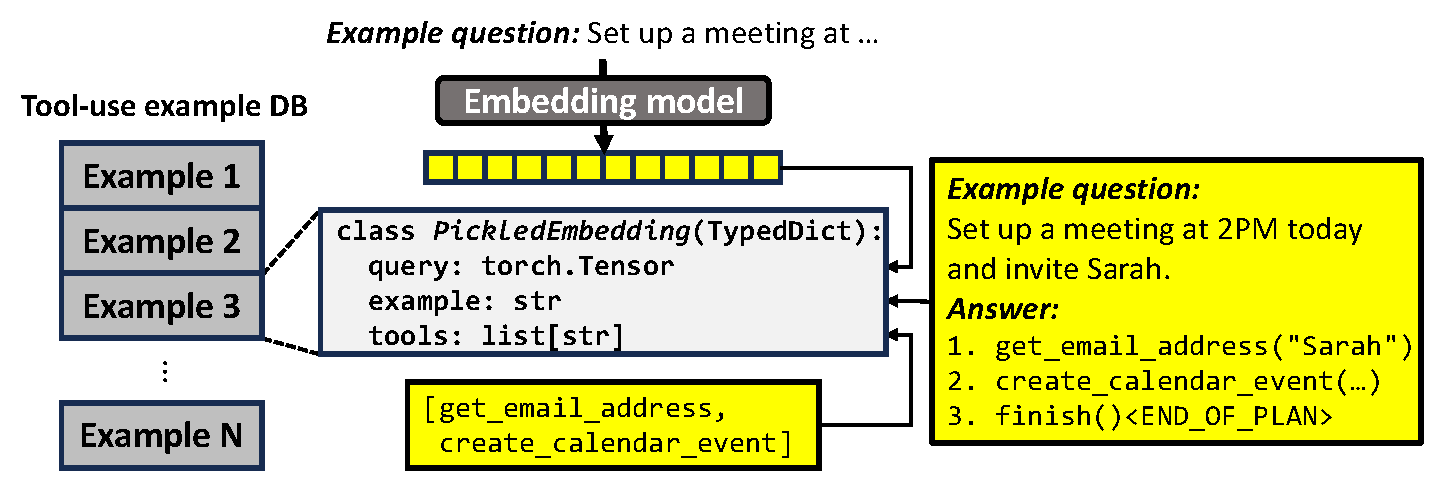
\includegraphics[width=\columnwidth]{./fig/offline_tool-use_example_database}} \\
\subfloat[Tool retrieval]
{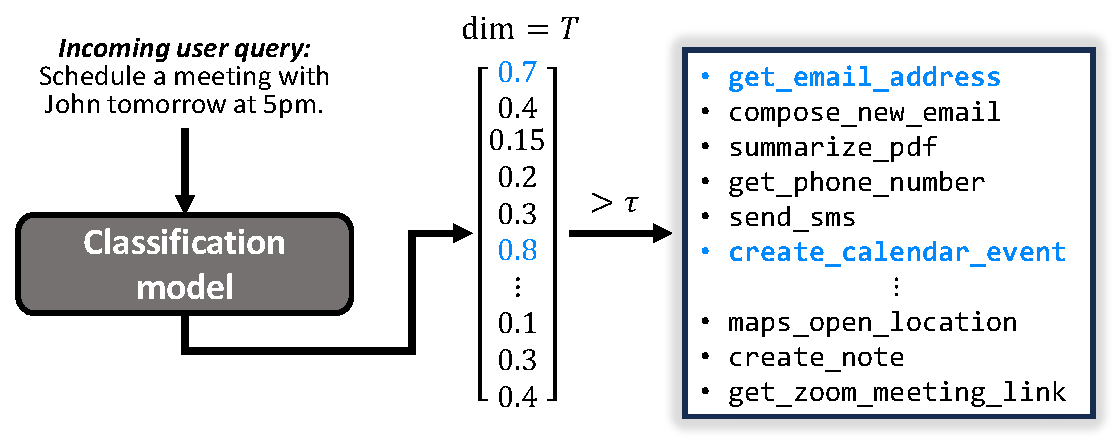
\includegraphics[width=\columnwidth]{./fig/tool_retrieval}} \\
\subfloat[Tool-use example (few-shot example) retrieval]{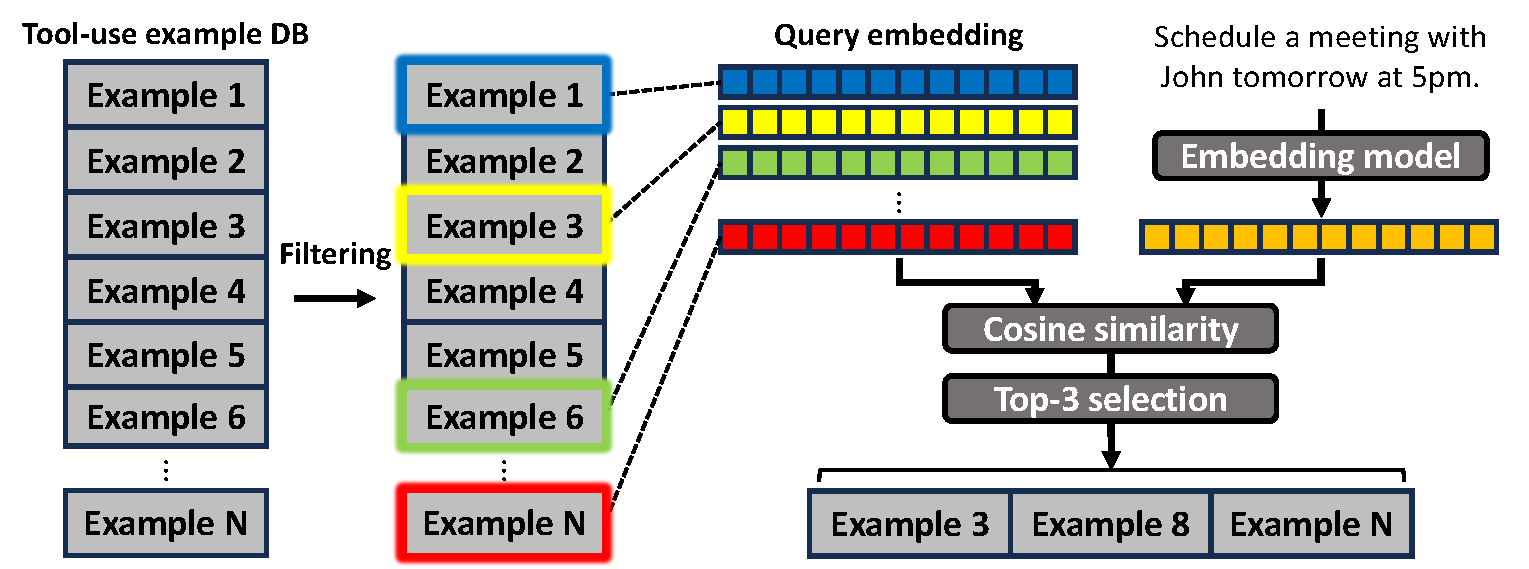
\includegraphics[width=\columnwidth]{./fig/tool-use_example_retrieval}} \\
\caption{
Illustration of the ToolRAG process.
}
\Description{Illustration of the ToolRAG process.}
\label{fig:toolrag}
\end{figure}


{\bf On-device LLMs.} AI functionalities are now available on edge devices, appearing in various forms like voice transcription~\cite{apple_intelligence}, Circle-to-Search~\cite{circle_to_search}, and personal assistants~\cite{siri,bixby,gemini_assistant}. Among them, LLMs are increasingly being deployed at the edge, due to their powerful performance. To power edge workloads, compact LLMs for resource-constrained devices have emerged~\cite{gemini_nano,afm}. Hardware accelerators~\cite{cambricon_llm,edge_moe,edgemoe,edgellm,clone,decdec} and deployment schemes~\cite{llm_in_a_flash,edgelora,crosslm,xpert} for on-device LLMs have also been proposed, driving the integration of on-device LLMs into everyday life.

{\bf On-device agents.} On-device agents make use of on-device LLMs to power local agents executing entirely on the user’s device. This design mitigates the security and privacy risks inherent in cloud-based solutions. The local LLM processes user requests (e.g., setting reminders) by invoking OS or third-party APIs and completing tasks fully on-device. Among existing systems~\cite{siri, bixby, gemini_assistant}, TinyAgent~\cite{tinyagent} is an open-source macOS agent that fine-tunes LLMs for agentic tasks. It also introduces ToolRAG (Tool Retrieval Augmented Generation)~\cite{tinyagent_toolrag} for efficient tool and example selection.

{\bf Tool choice and tool-use examples.} ToolRAG comprises three components: (i) offline preparation of a tool-use example database, (ii) runtime tool retrieval, and (iii) tool-use example retrieval. A diverse set of user queries is collected offline. Each query is annotated with (1) a fixed-dimension text embedding, (2) the example plan to handle the query, and (3) the set of tools needed to complete the task. Each database entry is stored as a tuple of these three elements: (\texttt{query}, \texttt{example}, \texttt{tools}) in \fig{fig:toolrag}(a).

At runtime, the user query is fed into a lightweight classification model (\fig{fig:toolrag}(b)). This model outputs a probability score for each of the $T$ available tools. A threshold of $\tau$ is applied to these scores, retaining only tools whose probability exceeds $\tau$. This filtering ensures that only the most relevant tools (e.g., \texttt{get\_email\_address} and \texttt{create\_calendar\_event}) are considered. Next, the tool-use example database is filtered, leaving out entries that include tools not selected by the classification model. The cosine similarities between the user's query embedding and each embedding in the filtered tool-use example database are computed. The top-$K$ examples with the highest similarity scores are retrieved (\fig{fig:toolrag}(c)). Finally, the Planner prompt is assembled by combining: (1) detailed descriptions of the selected tools, (2) usage guidelines, and (3) the retrieved tool-use examples ($K=3$ in \fig{fig:plan-out_agents}). Overall, ToolRAG constructs a prompt with highly relevant examples, enabling the on-device agent's Planner to generate better execution plans to accomplish the request.

The mechanism of dynamic tool selection and contextual example retrieval in ToolRAG reflects a broadly adopted paradigm in agent design~\cite{mcp, rag_mcp, toolformer, hugginggpt, llama3}. Agent systems often use similar workflows to constrain their action spaces and guide generation with task-specific examples. For example, the Model Context Protocol (MCP)~\cite{mcp}, an emerging open-source standard for LLM tool access driven by Anthropic, OpenAI, and Google, specifies that tool descriptions and usage examples be provided to the model. Likewise, Google’s Function Calling guide for Gemini~\cite{google_dev_function_calling, hera_agent} recommends the filtering of available functions based on conversational context before issuing calls. These shared design principles demonstrate that dynamic tool selection and tool-use example retrieval is not unique to ToolRAG, but a widely employed design paradigm in designing agentic systems.


\subsection{LLM Inference Optimization Methods} \label{sect:llm_optimization}


\begin{figure}[t!] \centering
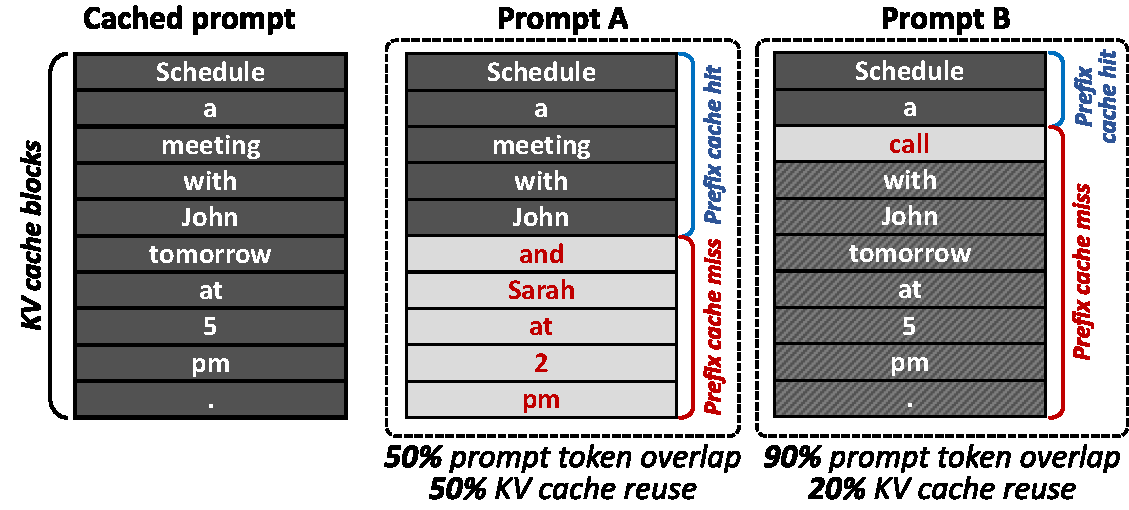
\includegraphics[width=\columnwidth]{./fig/prefix_caching} \\
\caption{
Illustration of applying prefix caching. Even though there exists substantial overlap between prompt B and the cached prompt, an early token mismatch limits the KV cache reuse.
}
\Description{Illustration of applying prefix caching.}
\label{fig:prefix_caching}
\end{figure}


LLM inference occurs in two stages: prefill and decode. During the prefill stage, the input prompt tokens are processed to populate the key-value (KV) cache, whose length grows with the number of tokens seen. In the decode stage, the model runs autoregressively, generating one token per step. Generally, prefill is compute-intensive, whereas decode is bounded by memory bandwidth~\cite{splitwise, pod_attention, sarathi, sarathi_serve, distserve}. Consequently, the latencies of conversational workloads running on cloud-based high-end GPU servers are known to be dominated by the decode stage (e.g., $>$ 95\% in \cite{wsc_llm, fdc, cent}).

{\bf Prefix caching.} In Transformer-based LLMs, each token attends only to preceding tokens. Therefore, when two inputs share a common prefix, they can reuse the same KV cache \textit{up to the first mismatched token.} \textit{Prefix caching}~\cite{vllm} exploits this by precomputing KV caches for shared prefixes, reducing prefill latency roughly proportional to the portion of cached tokens (i.e., amount of saved computation). As shown in \fig{fig:prefix_caching}, this technique works for prefixes of any length, but cache reuse halts at the first token mismatch, even if subsequent tokens are identical. Throughout this paper, \textit{cacheable tokens} refer to portions of prompts that prefix caching can be applied to with a single static prompt, and \textit{uncacheable tokens} refer to portions of prompts that cannot benefit from prefix caching due to an early token mismatch.

{\bf Speculative decoding.} An LLM's decode stage is memory bandwidth-bound because of its autoregressive, one-token-at-a-time nature, yielding low compute intensity. \textit{Speculative decoding}~\cite{specdec, sps} addresses this limitation by producing multiple \textit{draft tokens} per pass. \fig{fig:specdec} outlines the process, which uses a faster, less accurate \textit{draft model} to aid the generation of a slower, more accurate \textit{target model}.

First, the draft model autoregressively generates $N$ draft tokens (\circlednum{1}) with $N$ sequential forward passes. Next, the target model inputs the most recent token (\textit{``Schedule''}) concatenated with the $N$ draft tokens (\textit{``a'', ``meeting'', ``with'', ``Sarah''}) and enters the \textit{verification phase}. Here, for each draft token, the target model’s output logits and the draft model’s logits are compared, determining which tokens are accepted. The first mismatch (\textit{``Sarah''}) and all subsequent drafts are discarded (\circlednum{2}). Finally, the accepted draft tokens and the target model’s chosen next token (\textit{``John''}) form the input for the next speculation round (\circlednum{3}). Speculative decoding has been mathematically proven to yield outputs of comparable quality to standard autoregressive generation~\cite{specdec, sps}.
